I förra kapitlet togs en differentialekvation fram som beskriver vårt system som en relation mellan insignalen och utsignalen. Utifrån denna differentialekvation kan nu olika systemegenskaper tas fram som gör det möjligt att analysera systemet. Systemet kommer regera olika beroende på systemparametrarna, exempelvis kommer linan svänga olika beroende på vikten av personen på linan. 

Systemanalysen kommer titta närmare på följande funktioner: systemfunktionen, impulssvaret, stegsvaret, rampsvaret, frekvensfunktionen samt amplitud- och faskaraktäristiken.
Vissa av dessa funktioner tas fram med hjälp av olika transformer som existerar i frekvensdomänen vilket kommer diskuteras i nästa kapitel.

\textbf{(ny sida här för att få figuren på nästa sida att komma på rätt ställe, kanske går att fixa senare)(lägg in en passande bild istället?)}

\newpage
\subsection{Frekvensdomänen}
Tidigare i rapporten har vi betraktat insignalen och utsignalen som funktioner av tid. Vi kommer nu även betrakta hur signalerna beter sig i frekvensdomänen där man istället kollar på vilka frekvenser en signal är uppbyggd av.

Exempelvis kan signalen $x(t)=3sin(2t) + sin(4t)$ ses som summan av två amplituder i tidsdomänen. I frekvensdomänen skulle den dock vara uppdelad i dess frekvenskomponenter, i detta fall två komponenter vid frekvenserna $2$ och $4$. Detta visas grafiskt i figuren nedan.

\begin{figure}[h] % h = here
    \centering
    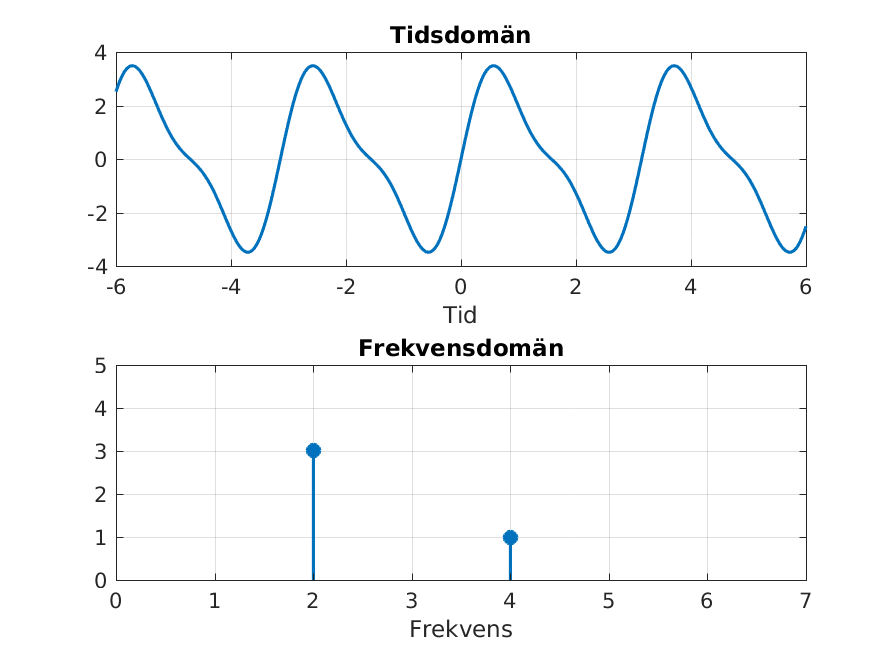
\includegraphics{bilder/tid_vs_frekvens_exempel}
    \caption{Tidsdomänen och frekvensdomänen av signalen $x(t)=3sin(2t)+sin(4t)$}
    \label{fig:tid_vs_frekvens_exempel}
\end{figure}

För systemanalysen kommer olika transformer som överför funktioner från tidsdomänen till frekvsensdomänen att användas, speciellt Laplacetransformen och Fouriertransformen.
Laplacetransformen är ett vanligt verktyg för att lösa differentialekvationer. För att ta sig tillbaka till tidsdomänen från frekvensdomänen kan inverstransformer appliceras.

\subsection{Systemfunktion}
Systemfunktionen, $H(s)$, beskriver förhållandet mellan utsignalen och insignalen i frekvensdomänen. Detta betyder att man kan räkna ut en utsignal om man vet insignalen i frekvensdomänen och systemfunktionen. 
Detta går också att göra i tidsdomänen med faltning men det är oftast enklare att utföra beräkningen i frekvensdomänen.

För att beräkna systemfunktionen kommer hela differentialekvationen för systemet att Laplacetransformeras till frekvensdomänen. Det finns då två versioner av Laplacetransformen som kan användas: den enkelsidiga och den dubbelsidiga.
Eftersom vårt system är kausalt, alltså att utsignalen inte beror på på framtida insignaler så kommer den enkelsidigia transformen att användas.
Den enkelsidiga Laplacetransformen för en funktion $x(t)$ definieras som:
$$X(s) = \mathcal{L}\big\{x(t)\big\} = \int\limits_{0-}^{\infty} x(t)e^{-st}\,dt$$
där s är en komplexvärd frekvens vanligtvis betecknad $s=\sigma+j\omega$.
Här används versaler för att beteckna funktioner i frekvensdomänen.
Denna transform behöver inte vara definierad för alla $s$ utan kan divergera i vissa fall. Därför är det viktigt att säga var den transformerade funktionen är definierad. 

Eftersom dessa integralberäkningar kan bli både långa och krångliga kommer vi i denna rapport använda tabellerna i häftet \textit{Formler \& Tabeller}\footnote{Sune Söderkvist, \textit{Formler \& Tabeller}, 4:e upplagan (2007)} för att beräkna Laplacetransformerna.
För att transformera differentialekvationen kommer följande samband för derivering i tidsdomänen att användas enligt tabell 18.7:
$$\mathcal{L}\bigg\{\frac{dy(t)}{dt}\bigg\} = sY(s)-y(0-)$$
Då vårt system är energifritt är alla $y(0-)$-termer lika med noll. Vår differentialekvation kan alltså Laplacetransformeras enligt:
$$ \mathcal{L}\bigg\{m\displaystyle\frac{d^2y(t)}{dt^2} + c\displaystyle\frac{dy(t)}{dt} + ky(t)\bigg\}= \mathcal{L}\bigg\{x(t)\bigg\} $$
\begin{center}$ \Longleftrightarrow \bigg/$ Tabell $18.7$, $18.8\,\bigg/$ \end{center}
$$ \Longleftrightarrow\, ms^2Y(s)+csY(s)+kY(s)=X(s)$$

Från ekvationen ovan kan nu systemfunktionen $H(s)$ bestämmas då den definieras som kvoten mellan utsignalen och insignalen i frekvensdomänen. Genom att bryta ut termen $Y(s)$ i vänsterledet och sedan dela med $X(s)$ och $s$-polynomet i båda led ges följande: 
$$H(s)=\frac{Y(s)}{X(s)}=\frac{1}{ms^2+cs+k}$$
\newline

\subsubsection{Pol-nollställediagram}
Utifrån systemfunktionen kan nu flera egenskaper om systemet tas fram. Oftast är det intressant att studera nollställena för polynomen i systemfunktionen. Täljarpolynomets rötter kallas systemfunktionens nollställen medan nämnarpolynomets rötter kallas systemfunktionens poler. Man kan direkt se att systemfunktionen inte har några nollställen då täljarpolynomet inte har några rötter. För att hitta polerna måste rötterna till nämnarpolynomet hittas, detta kan till exempel göras med pq-formeln:
$$ms^2+cs+k=0$$
$$\Longleftrightarrow s=-\frac{c}{2m}\pm \sqrt{\bigg(\frac{c}{2m}\bigg)^2-\frac{k}{m}}$$

Här uppstår 3 potentiella fall för poler beroende på uttrycket i kvadratroten, den så kallade diskriminanten.

\begin{itemize}
    \item Om diskriminanten är positiv bildas två skilda reella poler. Kravet är då: 
    $$ \bigg(\frac{c}{2m}\bigg)^2-\frac{k}{m} > 0 \,\,\, \Longleftrightarrow\,\,\, \frac{c^2}{4m} > k $$   
    \item Om diskriminanten är noll bildas en reell dubbelpol. Kravet för dubbelpolen är: 
    $$ \bigg(\frac{c}{2m}\bigg)^2-\frac{k}{m} = 0 \,\,\, \Longleftrightarrow\,\,\, \frac{c^2}{4m} = k $$
    \item Om diskriminanten är negativ bildas två komplexkonjugerade poler. Kravet för komplexa poler är: 
    $$ \bigg(\frac{c}{2m}\bigg)^2-\frac{k}{m} < 0 \,\,\, \Longleftrightarrow\,\,\, \frac{c^2}{4m} < k $$
\end{itemize}

Som nämnts innan behöver inte Laplacetransformen vara definierad för alla $s$. Var transformen konvergerar i det komplexa planet bestäms av den reella delen av $s$ och kallas konvergensområdet. För kausala system får man högersidiga konvergensområden i det komplexa planet. Då bestäms konvergensområdets vänstra gräns av den pol som är längst till höger. För vårt system får vi två fall för detta beroende på var polerna är placerade.
\begin{itemize}
    \item Om vi har en reell dubbelpol eller komplexkonjugerade poler så är konvergensområdet:
    $$ Re\{s\} > -\frac{c}{2m} $$
    \item Om vi har två skilda reella poler så blir konvergensområdet:
    $$ Re\{s\} > -\frac{c}{2m}+\sqrt{\bigg(\frac{c}{2m}\bigg)^2-\frac{k}{m}} $$
\end{itemize}

För att få en bättre förståelse av systemfunktionen kommer poler, nollställen och konvergensområdet visas grafiskt i ett pol-nollställediagram. För detta behöver även nivånkonstanten $K$ bestämmas. Denna fås genom att bryta ut koefficienterna för den högsta graden av $s$ i täljar- och nämnarpolynomet. I vårt fall är denna alltid:
$$K=\frac{1}{m}$$
Nedan visas pol-nollställediagramen för de 3 olika fallen för polerna. Enligt standardnotation representerar kryssen poler och cirklar nollställen, dock uppstod inga nollställen. De rödsträckade området är konvergensområdet.

\begin{figure}[H] % h = here
    \centering
    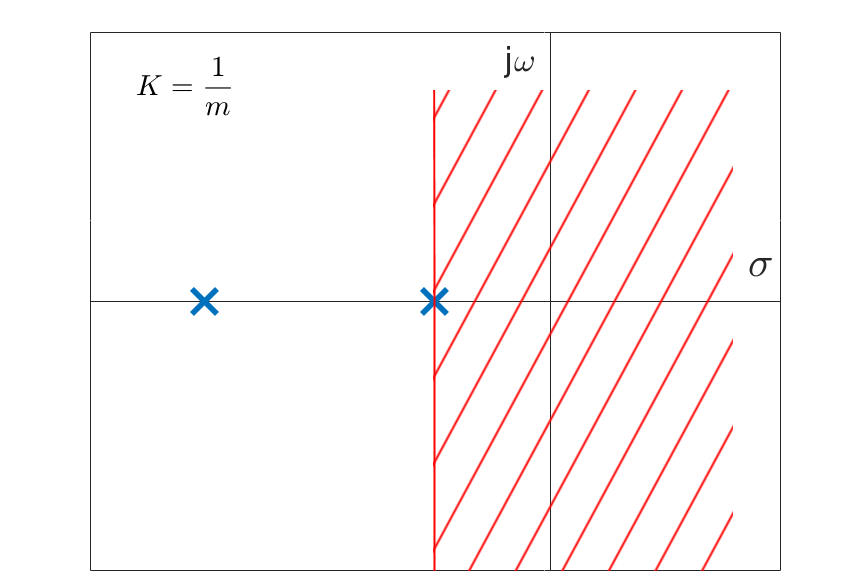
\includegraphics[scale=0.33]{bilder/pol_nollstallediagram_2_poler}
    \caption{Pol-nollställediagram för 2 skilda reella poler}
    \label{fig:pol_nollstallediagram_2_poler}
\end{figure}
\begin{figure}[H] % h = here
    \centering
    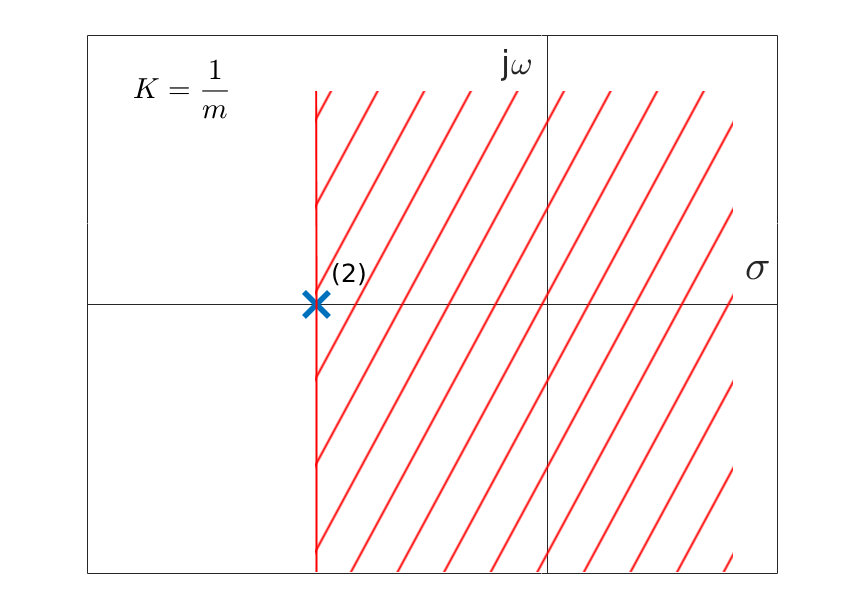
\includegraphics[scale=0.33]{bilder/pol_nollstallediagram_dubbelpol}
    \caption{Pol-nollställediagram för en reell dubbelpol}
    \label{fig:pol_nollstallediagram_dubbelpol}
\end{figure}
\begin{figure}[H] % h = here
    \centering
    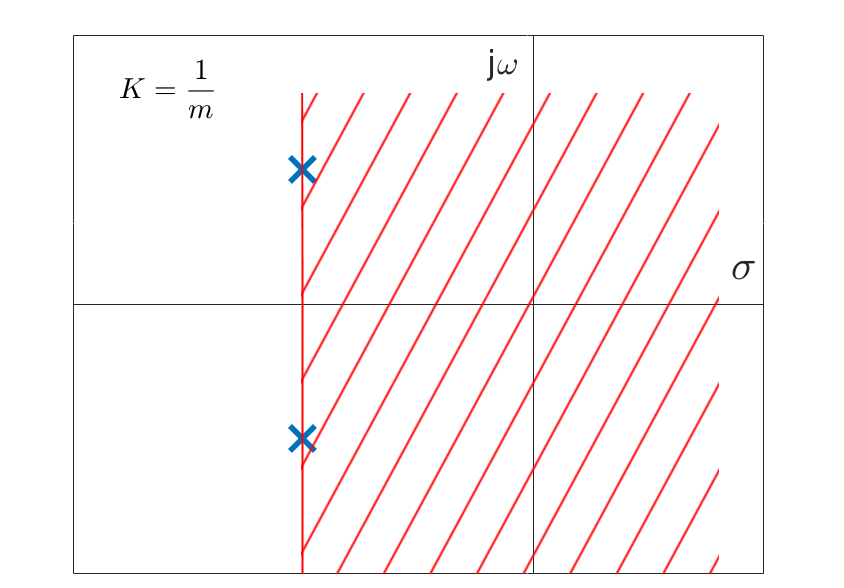
\includegraphics[scale=0.33]{bilder/pol_nollstallediagram_komplexa_poler}
    \caption{Pol-nollställediagram för två komplexkonjugerade poler}
    \label{fig:pol_nollstallediagram_komplexa_poler}
\end{figure}
 
\newpage
\subsection{Impulssvar}
Vi ska nu se hur vårt system reagerar olika på typer en insignaler. En vanligt signal som studeras är enhetsimpulsen också kallad Dirac-pulsen, $\delta(t)$. 
Enhetsimpulsen är noll för alla värden $t\ne 0$. Vid $t = 0$ är den oändligt stor så att dess area är lika med $1$. Det är svårt att föreställa hur detta skulle representera sig fysikalisk i vår modell. Ett ungefärligt exempel skulle vara då man släpper en tennisboll från en hög höjd som träffar personen på huvudet och studsar bort. 

Impulssvaret $h(t)$ är utsignalen då ett system tar emot en enhetsimpuls som insignal. Denna kan räknas ut genom att inverstransformera systemfunktionen $H(s)$. Vi kommer återigen att använda tabeller för dessa beräkningar då integralerna är jobbiga att räkna ut. Man får istället problemet att skriva om uttrycken så att de matchar något i tabellen. Då det finns 3 uppsättningar av poler kommer implussvaret för dessa räknas ut separat.

\begin{itemize}
    \item Vid 2 skilda reella poler kan vi faktorisera rötterna i nämnarpolynomet och partialbråksuppdela för att hitta en lämplig inverstransform.
    
    $$H(s)=\frac{1}{m} \cdot \frac{1}{s^2+\frac{cs}{m}+\frac{k}{m}}=\Bigg/ \,\alpha=\frac{c}{2m}\,\,,\,\,\, \omega_0=\sqrt{\bigg(\frac{c}{2m}\bigg)^2-\frac{k}{m}} \,\,\Bigg/$$
    $$=\frac{1}{m} \cdot \frac{1}{\big(s+\alpha-\omega_0\big)\big(s+\alpha+\omega_0\big)}  = \, \frac{1}{2m\omega_0} \Bigg(\frac{1}{s+\alpha-\omega_0}-\frac{1}{s+\alpha+\omega_0}\Bigg)$$
    \begin{center}$ \Longleftrightarrow \bigg/$ Tabell $19.12\,\bigg/$ 
    $\Longleftrightarrow h(t)=\dfrac{1}{2m\omega_0}\bigg(e^{-(\alpha-\omega_0)t}-e^{-(\alpha+\omega_0)t}\bigg)u(t)$ \end{center}
    
    \item Vid reell dubbelpol kvadratkompletteras nämnarpolynomet och utnyttjas att
    $\dfrac{k}{m}-\dfrac{c^2}{4m^2}=0$.
    $$ H(s)= \frac{1}{m} \cdot\frac{1}{\big(s+\frac{c}{2m}\big)^2+\big(\frac{k}{m}-\frac{c^2}{4m^2}\big)} = \frac{1}{m} \cdot \frac{1}{\big(s+\frac{c}{2m}\big)^2}$$
    \begin{center}
    $ \Longleftrightarrow \bigg/ \alpha=\dfrac{c}{2m}\,,\,$ Tabell $19.15\,\bigg/ \Longleftrightarrow h(t)=\dfrac{1}{m} \cdot te^{-\alpha t}\,u(t)$
    \end{center}
    
    \item För komplexkonjugerade poler kvadratkompletteras nämnarpolynomet precis som innan. Sedan anpassas uttrycket med hjälp av förlängning för att överrensstämma med tabellen.
    $$H(s)=\frac{1}{m} \cdot \frac{1}{\big(s+\frac{c}{2m}\big)^2+\big(\frac{k}{m}-\frac{c^2}{4m^2}\big)} = \Bigg/\, \,\alpha=\frac{c}{2m}\,\,,\,\,\,\omega_0=\sqrt{\frac{k}{m}-\frac{c^2}{4m^2}} \,\,\,\Bigg/ $$
    \begin{center}
    $=\dfrac{1}{m\omega_0} \cdot \dfrac{\omega_0}{(s+\alpha)^2+\omega_0^2} \,\,\Longleftrightarrow \bigg/$ Tabell $19.23\,\bigg/\Longleftrightarrow\,\, h(t)=\dfrac{1}{m\omega_0} \cdot e^{-\alpha t} \sin(\omega_0 t)u(t)$
    \end{center}
\end{itemize}

\subsubsection{Val av systemparametrar}
Innan de 3 olika impulssvaren ska ritas ut (\textbf{finns bättre ord här}) så ska några standarder (\textbf{finns bättre ord här}) sättas för systemparametrarna. Dessa bestämmer hur systemen beter sig och är i vårt fall de 3 hittills obestäma konstanterna: massan  $m$, fjäderkonstanten $k$ och dämpningskonstanten $c$. För att se hur olika parameteruppsättningar skilljer sig åt komma vi variera dessa en i taget medan de andra två behålls konstanta. (\textbf{Kom ihåg, två parameteruppsättningar = två olika system != samma system med olika variabler i})

Valet av systemparametrar baseras på scenariot som beskriv i inledningen. Den första parametern som kommer bestämmas är massan. Denna bestäms vara $75$ kg (\textbf{ska detta skrivas ihop till 75kg?}),  vilket är den ungefärliga medelvikten hos svenska män och kvinnor \href{http://www.scb.se/sv_/Hitta-statistik/Statistik-efter-amne/Levnadsforhallanden/Levnadsforhallanden/Undersokningarna-av-levnadsforhallanden-ULFSILC/12202/2012A02B/Behallare-for-Press/6-kilo-mer-man-och-4-kilo-mer-kvinna/}{\textbf{REFERENS}}.
Nästa parameter är dämpningskonstanten vilket härleds från differentialekvationen i viloläget, där konstanten $k$ kan skrivas som:
$$k=\frac{mg}{y_0}$$
Vi måsta alltså bestäma en rimlig utdragning av linan i viloläget för att sedan räkna ut $k$. Vi anser att en rimligt utdragning av linan är $1$ m (\textbf{alt 0.5 m}) efter att studerat bilder och filmklipp av riktiga lindansare. Vi antar att jordens tyngdacceleration kan approximeras till $g=9.82$. Då blir fjäderkonstanten:
$$k=\frac{75 \cdot 9.82}{1}\approx 737 \text{ N/m}$$

Sist har vi dämpningskonstanten $c$ som är ganska svår att bestämma. Denna kan bestämas med till exempel experiment där man mäter hur mycket systemet dämpar en insignal. Detta är inte möjligt i vårt fall och vi behöver därför resonera oss fram till ett rimligt värde. Dämpningskonstanten kommer bestäma typen av system alltså vilken typ av poler som bildas. Vi vill att systemet dämpar insingaler så lindansaren har lättare att balansera sig på linan. Man vill fortfrande ha lite gung i linan men den vara väldigt begränsad (\textbf{Typ bullshit de jag just sa, men håller ni med?}). Vi får denna effekt då vi har 2 skilda reella poler och kravet för det var:
$$\frac{c^2}{4m} > k $$
Löser vi ut $c$ och stoppar in värdena från innan får vi:
$$c>\sqrt{4km}=\sqrt{4\cdot 737\cdot 75} \approx 740$$
Vi väljer att $c=1000$ \textbf{ENHET HÄR} för att skapa heltalsrötter i andra ekvationer. (\textbf{dummaste motiveringen egentligen..., den skapar inte ens hela rötter bara approximativa löl}).

Standardparameteruppsättningen (bästa ordet jag kan komma på) kan sammanfattas (till? som?)

$\begin{cases}
m=75 \text{ kg} \\
k=737 \text{ N/m} \\
c=1000 \text{ ENHET HÄR}
\end{cases}$


\textbf{När 75kg vs 75 kg har bestämst: gå tillbaka till slutet av kapitel 1 och fixa de där också}.

kanske försöka koppla variationen till verkligheten, massa = lättare/tyngre person. fjäder = lättare spänd lina(?). dämpningskonstant = annat material på lina (också ???).
nämn standardvariation här eller senare?

\subsubsection{Variation av impulssvaret}
Hitta en bättre titel. kanske ''variation av impulssvaret''?




\newpage
\subsection{Stegsvar}
En annan insignal som vi ska studera är enhetssteget $u(t)$. Detta är en plötslig förändring av insignalen från $0$ till $1$ enligt:
$$u(t)=\begin{cases} 1, & \text{om } t \ge 0 \\ 0, & \text{om } t < 0\end{cases}$$
När ett system matas med ett enhetssteg så får man stegsvaret $g(t)$ som utsignal. Eftersom vårt system är linjärt kan denna utsignal beräknas genom att falta enhetssteget med impulssvaret som har beräknats innan. Denna uträkning kan sedan förenklas till en integral över bara impulssvaret enligt:
$$g(t)=(u*h)(t)=\int\limits_{-\infty}^{\infty}h(\tau)\,u(t-\tau)\,d\tau=\int\limits_{-\infty}^{t}h(\tau)\,d\tau$$
(\textbf{vad skulle detta vara i vårt system})
Då vi har 3 typer av generella system så har vi räknat ut 3 olika impulssvar och kommer därför också räkna ut 3 olika stegsvar. ... behåller vi konstanterna som valdes då impulsvaren räknades ut. Eftersom alla impulssvar har en term av enhetsteget i sig så blir faltning alltid $0$ då $t < 0$. Här beräknar vi vad som händer då $t \ge 0$.

\begin{itemize}
    \item Vid 2 skilda reella poler så kan vi direkt integrera exponentialfunktionerna.
    $$g_1(t)=\int\limits_{-\infty}^{t}\dfrac{1}{2m\omega_0}\bigg(e^{-(\alpha-\omega_0)\tau}-e^{-(\alpha+\omega_0)\tau}\bigg)u(\tau)\,d\tau
    =\dfrac{1}{2m\omega_0}\int\limits_{0}^{t}\bigg(e^{-(\alpha-\omega_0)\tau}-e^{-(\alpha+\omega_0)\tau}\bigg)\,d\tau$$
    $$=\dfrac{1}{2m\omega_0}\bigg[\frac{e^{-(\alpha+\omega_0)\tau}}{(\alpha+\omega_0)}-\frac{e^{-(\alpha-\omega_0)\tau}}{(\alpha-\omega_0)} \bigg]_{\tau=0}^{\tau=t}
    =\dfrac{1}{2m\omega_0(\alpha^2-\omega_0^2)}\bigg((\alpha-\omega_0)e^{-(\alpha+\omega_0)t}-(\alpha+\omega_0)e^{-(\alpha-\omega_0)t}+2\omega_0\bigg)$$
    \\
    \item Vid dubbelpol så används partiell integration en gång för lösa integralen.
    $$g_1(t)=\dfrac{1}{m}\int\limits_{0}^{t}\tau e^{-\alpha \tau}\,d\tau=
    \dfrac{1}{m} \bigg[\dfrac{\tau e^{-\alpha \tau}}{-\alpha}\bigg]_{\tau=0}^{\tau=t}+\dfrac{1}{m\alpha}\int\limits_{0}^{t}e^{-\alpha \tau}\,d\tau$$
    $$=-\dfrac{1}{m\alpha^2}\alpha te^{-\alpha t}+\dfrac{1}{m\alpha}\bigg[\dfrac{e^{-\alpha \tau}}{-\alpha}\bigg]_{\tau=0}^{\tau=t}=
    \dfrac{1}{m\alpha^2}\bigg(1-e^{-\alpha t}(\alpha t+1)\bigg)$$
    \newpage
    \item Vid komplexkonjugerade poler så används upprepad partiell integraion. Då får man tillbaka uttrycket som man hade från början och kan på så sätt lösa ut stegsvaret.
    $$g_1(t)=\dfrac{1}{m\omega_0}\int\limits_{0}^{t} e^{-\alpha \tau} \sin(\omega_0 \tau)\,d\tau
    =\dfrac{1}{m\omega_0}\bigg[\dfrac{e^{-\alpha \tau}\sin(\omega_0 \tau)}{-\alpha}\bigg]_{\tau=0}^{\tau=t}+\dfrac{1}{m\alpha}\int\limits_{0}^{t} e^{-\alpha \tau} \cos(\omega_0\tau)\,d\tau$$
    $$=-\dfrac{e^{-\alpha t}\sin(\omega_0 t)}{m\omega_0\alpha}+\dfrac{1}{m\alpha}\bigg[\dfrac{e^{-\alpha \tau}\cos(\omega_0 \tau)}{-\alpha}\bigg]_{\tau=0}^{\tau=t}-\dfrac{\omega_0}{m\alpha^2}\int\limits_{0}^{t}e^{-\alpha \tau} \sin(\omega_0 \tau)\,d\tau$$
    $$=-\dfrac{e^{-\alpha t}\sin(\omega_0 t)}{m\omega_0\alpha}+\dfrac{1-e^{-\alpha t}\cos(\omega_0 t)}{m\alpha^2}-\dfrac{\omega_0^2}{\alpha^2}\,g_1(t)$$
    
    $$\Longleftrightarrow g_1(t)
    =\dfrac{\omega_0-e^{-\alpha t}(\alpha\sin(\omega_0 t)+\omega_0\cos(\omega_0 t))}{m\omega_0(\alpha^2+\omega^2)}$$
\end{itemize}
Eftersom dessa tre stegsvar bara gäller då $t\ge 0$ så kommer de multipliceras med enhetssteget för ett fullständigt stegsvar enligt:
$$g(t)=g_1(t)\cdot u(t)$$
Detta ger att stegsvaren för reella poler, dubbelpol respektive komplexa poler blir:

$\begin{cases}
g(t)=\dfrac{(\alpha-\omega_0)e^{-(\alpha+\omega_0)t}-(\alpha+\omega_0)e^{-(\alpha-\omega_0)t}+2\omega_0}{2m\omega_0(\alpha^2-\omega_0^2)}\,u(t) \\\\
g(t)=\dfrac{1-e^{-\alpha t}(\alpha t+1)}{m\alpha^2}\,u(t) \\\\
g(t)=\dfrac{\omega_0-e^{-\alpha t}(\alpha\sin(\omega_0 t)+\omega_0\cos(\omega_0 t))}{m\omega_0(\alpha^2+\omega_0^2)}\,u(t)
\end{cases}$

\textbf{Förslag för förtydligande: Döpa om alla $h(t)$ till $h_r(t)$, $h_d(t)$  och $h_k(t)$ för reella, dubbel och komplex, alt. $h_1(t), h_2(t), h_3(t)$}

\subsubsection{Variation av stegsvaret}
\newpage
\subsection{Rampsvar}
Är detta relevant?
((= Dampsvar?! det enda dampsvaret här är du....),förmodligen inte)
Tydligen är detta relevant även fast de aldrig kommer hända i verkligheten. Tack Lasse!

Tror detta kommer skippas pga tidsbirst och brist på plats
\newpage
\subsection{Stabilitet}
\textbf{Ska inte det här komma tidigare i rapporten????!?}

\textbf{Det har inte behövts innan. Först var de tänkt att vi skulle göra det under ''implussvaret'' för det är då vi vet att systemet är stabilt. Vi behöver att system är stabilt för att kunna ta fram fouriertransformen (frekvensfunktionen). NÄMN DETTA TYP DE FÖRSTA DU GÖR I DETTA KAPITEL}

Ett stabilt system är ett system där begränsade insignaler alltid ger begränsade utsignaler. Gäller detta inte (dvs att systemet är instabilt) innebär det att vid vissa insignalers som inte är oändligt stora får man en oändligt stor utsignal. I lindansarens fall skulle detta innebära att det vid någon frekvens (\textbf{finns bättre ord här, möjligt att impuls ger oändlig output?}) skulle uppstå resonans så att höjdavvikelsen hela tiden ökade (mot oändligheten). Om lindansaren råkade gunga vid just den frekvensen skulle sådan fart nås att linan skulle brista och lindansaren slungas av och troligen skada sig illa. Därför är det viktigt att vårt system är stabilt.

Ett instabilt system där det endast några få begränsade insignaler resulterar i obegränsade utsignaler kallas för marginellt stabilt. Om dessa insignaler är sådana som "aldrig" inträffar eller om man kan kompensera för dem så att de inte kan inträffa vore även ett marginellt stabilt system okej för lindansaren.

För att bestämma huruvida ett system är stabilt eller ej finns olika tillvägagångssätt. Ett sätt att bestämma detta är att titta på impulssvaret. Om impulssvaret är absolutintegrerbart så är systemet stabilt (\textbf{sats 3.42, måste detta visas/alt refereras till från boken? EHh du kan hänvisa till boken fast jag tar allt vi säger som typ fakta/underförstådda saker. Behöver vi ens ta upp det om vi ändå bara använder pol/-nollställediagrammet? Eller står det nånstans att man måste visa abs.integ.barhet? Nej egentligen inte, men jag tycker de visar på att vi förstår vad stabilitet betyder och att det finns flera sätt att visa det på}). Att impulssvaret är absolutintegrerbart innebär att:
$$\int\limits_{-\infty}^{\infty}\big|h(t)\big|\,dt < \infty$$
Ett annat sätt att bestämma om impulssvaret är stabilt är att titta på systemfunktionen och pol-/nollställena. Denna metod kan härledas från föregående metod (\textbf{Alltså sats 3.42}). Då gäller att ett kausalt LTI-system är stabilt om det har fler poler än nollställen och att samtliga poler befinner sig till vänster om imaginäraxeln ($j\omega$)(dvs att konvergensområdet innesluter imaginäraxeln). Som visats i 2.2 har vårt system fler poler än nollställen, och som kan ses i 2.2.1 och mer tydligt i Figur 4, 5 och 6 befinner sig samtliga poler alltid till vänster om imaginäraxeln. Alltså är vårt system stabilt. (\textbf{Givet att m!=0, är det nåt som ska nämnas någonstans överhuvudtaget elr är det ett trivial antagande? För att vårt system ska vara stabilt så krävs att  $m,k,c > 0$. Detta är uppenbart för att det är ett fysikaliskt och realiserbart system. Du kan nämna de kort om du vill})

(\textbf{Notes sen innan skrivandet av 2.6})

Var är stabilitet? (kanske mer viktigt: vad betyder stabilititet? im 12 btw)

Begränsasd insignal ger... begränsad utsignal

Absolutintegrerbart impulssvar....

jw-axeln i konvergensomrpdet....

vad betyder detta för vårat fysikaliska system? är det rimligt?
(detta är uppenbart men det drar ut vår rapport med 1-2 (du menar 7-18) rader, worth!)


\subsection{Frekvensfunktion}
$$H(\omega)=H(s)\bigg\rvert_{s=j\omega}=\dfrac{1}{m(j\omega)^2+cj\omega+k}$$

\subsection{Amplitud- och faskaraktäristik}


\subsection{Utsignal}

\subsection{SAKER SOM SKA KOLLAS DÅ ALLT ÄR KLART}
\begin{itemize}
    \item Vi blandar tex ''3'' och ''tre'' lite överallt. Använd en av dom (helst den som är korrekt http://dinsvenska.se/datum-tid-och-rakneord/ska-man-skriva-tal-med-siffror-eller-bokstaver/)
    \item Kolla ekvationerna, framför stora snedsträck används ibland ''='' och ibland ''$\Longleftrightarrow$''. Tror att vissa av dessa är fel.
    \item Ska vi använda dubbel- eller enkelpilar? 
    \item Fixa storleken på alla formler i rapporten
    \item Lös kommentarerna i kapitel 1.3 angående friktionen.
    \item Lägg till text för att läsaren ska tolka och förstå bättre under Bevis av linjäritet.
    \item Fråga en annan grupp om de kan läsa vår rapport och ge kommentarer (i utbyte att vi läser deras)
    \item Lägg till radbrytning där det ser snyggt ut
    \item Läs igenom i grupp
    \item Skriv ut och läs igen
\end{itemize}